\documentclass[12pt,a4paper,oneside]{report}
\usepackage{enumitem}
\usepackage{xcolor}
%\usepackage{sectsty}
\usepackage{longtable}
\usepackage{caption}
\usepackage{subcaption}
\usepackage{float}
\usepackage{graphicx}
\usepackage{tabularray}
\usepackage{array}
\usepackage{setspace}
\usepackage{tocloft}
\usepackage[nottoc]{tocbibind}
\usepackage{amsmath}
\usepackage{amsfonts}
\usepackage{amssymb}
\usepackage{makeidx}
\usepackage{multirow}
\usepackage[left=1in,right=1in,top=1in,bottom=1in]{geometry}
\usepackage[super,square,sort,comma,numbers]{natbib}
\usepackage[version=4]{mhchem}

%\chapternumberfont{\normalsize} 
%\chaptertitlefont{\LARGE}
%\sectionfont{\large}

\setlength{\extrarowheight}{2pt}

\renewcommand{\thefootnote}{\fnsymbol{footnote}}
\renewcommand{\contentsname}{\Large CONTENTS}
\renewcommand{\cftfigfont}{Figure }
\renewcommand{\cfttabfont}{Table }
\renewcommand{\cftdot}{}
\graphicspath{{./images/}}

\setcitestyle{square}
\pagenumbering{roman}
\date{}

\begin{document}
\thispagestyle{empty}
\begin{center}
{\Large  \MakeUppercase{\bf Automation of DevOps Processes}\\} 
\vspace{0.8cm}
{\Large  \MakeUppercase{\bf Long-Term Internship Report}\\}
\doublespacing
\vspace*{2.5cm}
{\normalsize \it A report submitted in partial fulfillment of the requirements for award of the Degree of\\
}
{\bf BACHELOR OF TECHNOLOGY }\\
{\bf in }\\
{\bf COMPUTER SCIENCE ENGINEERING }\\
{\bf by }\\
\vspace*{1cm}
{\bf\textcolor{blue} {BALINENI SREEDHAR NAIDU }}\\
{\bf \textcolor{blue}{ID: N180058}} \\
{\bf Under supervision of }\\
{\bf Mr. Venkata Narasimha Kowru, SaYukth}\\
{\bf Technologies Pvt Ltd,Hyderabad} \\
{\bf 11 Sep, 2023 to 15 Mar, 2024} \\ 
{\bf Major Project Guide: Mr. Kalapala Sravan Kumar } \\

\vspace*{0.8cm}
\begin{figure}[hbt]
\centering
\vspace*{0.6cm}
\centerline{
\includegraphics[scale=0.29]{images/rgukt.png}}
\end{figure}
\vspace*{0.3cm}
{\small \bf DEPARTMENT OF COMPUTER SCIENCE ENGINEERING}\\
{\small \bf RAJIV GANDHI UNIVERSITY OF KNOWLEDGE TECHNOLOGIES}\\
{\small \bf NUZVID, INDIA\\ }
\end{center}
\newpage
\thispagestyle{empty}
\vspace*{1cm}
\begin{center}{\large \bf DECLARATION}\end{center}
\vspace{1cm}
\setstretch{1.5}
\hspace{1cm}I, \textbf{Balineni Sreedhar Naidu}  hereby declare that the long-term project report is submitted for partial fulfilment of the requirements for the award of the degree of Bachelor of Technology in Computer Science Engineering of the Rajiv Gandhi University of Knowledge Technologies, Nuzvid is a bonafide work done by me under the supervision of\\ \textbf{Mr. Venkata Narasimha Kowru}, Team Leader at SaYukth Technologies Pvt Ltd,Hyderabad, and under the guidance of \textbf{Mr. Kalapala Sravan Kumar }. This submission represents my ideas in my own words and where ideas or words of others have been included, I have adequately and accurately cited and referenced the original sources. I also declare that I have adhered to the ethics of academic honesty and integrity and have not misrepresented or fabricated any data or idea or fact or source in my submission. I understand that any violation of the above will be a cause for disciplinary action by the institute and/or the University and can also evoke penal action from the sources which have thus not been properly cited or from whom proper permission has not been obtained. This report has not been previously formed as the basis for the award of any degree, diploma, or similar title of any other University.
\\
\vspace{1cm} \\
...............................\\
Internal Examiner :\\
Date : \\
\vspace{1cm} \\
\textbf{Balineni Sreedhar Naidu (N180058)}  



\newpage
\pagenumbering{roman}
\thispagestyle{empty}

\setstretch{1.25}
\begin{center}
{\large \bf DEPARTMENT OF COMPUTER SCIENCE ENGINEERING}\\
{\large \bf RAJIV GANDHI UNIVERSITY OF KNOWLEDGE TECHNOLOGIES,}
{\large \bf NUZVID, INDIA}\vspace{0.1cm}\end{center}

\begin{figure}[hbt]
\centering
\centerline{
\includegraphics[scale=0.25]{images/rgukt.png}}
\end{figure}

\begin{center} 
\addcontentsline{toc}{chapter}{Certificate}
{\Large  \textbf{CERTIFICATE}}\end{center}
\begin{spacing}{1.5}
This is to certify that the report entitled \textbf{"Automation of DevOps Processes"} submitted by \textbf{Balineni Sreedhar Naidu (N180058)} to the Rajiv Gandhi University of Knowledge Technologies, Nuzvid in partial fulfilment of the requirements for the award of the Degree of Bachelor of Technology in Computer Science Engineering is a bonafide record of the project work carried out by him under our guidance and supervision. This report in any form has not been submitted to any other University or Institute for any purpose.\end{spacing}
\vspace{2cm}
\noindent
\begin{tabular}[t]{@{}l}
\textbf{Mr. Kumar Anurupam }\\ Internal Supervisor\\Professor\\Dept. of Computer Science Engineering \\RGUKT NUZVID
\end{tabular}
\hfill
\begin{tabular}[t]{@{}r}
\textbf{Mr. R. Siva Narayana}\\External Supervisor\\Asst.Professor\\Dept. of Computer Science Engineering\\RGUKT NUZVID
\end{tabular}



\vspace{2cm}
\noindent
\begin{tabular}[t]{@{}l}
\textbf{Mr. B. Mahalakshmi Rao}\\External Supervisor\\Asst.Professor\\Dept. of Computer Science Engineering\\RGUKT NUZVID
\end{tabular}
\hfill
\begin{tabular}[t]{@{}r}
\textbf{Dr. D.V. Nagarjuna Devi}\\Head of the Department\\Dept. of Computer Science Engineering \\RGUKT NUZVID
\end{tabular}

% \vspace{2cm}
% \noindent
% \begin{tabular}[t]{@{}l} 
% \textbf{Mr. S. Chiranjeevi}\\Head of the Department\\Dept. of Computer Science Engineering \\RGUKT NUZVID
% \end{tabular}
% \hfill
% \begin{tabular}[t]{@{}r} 
% \end{tabular}




\newpage

\thispagestyle{empty}
\vspace*{3cm}
\addcontentsline{toc}{chapter}{Acknowledgement}
\begin{center}  {\large \bf ACKNOWLEDGEMENT}\end{center}
\vspace{1cm}
\setstretch{1.5}
\hspace{1cm}We express our sincere gratitude towards our Team Leader \textbf{Mr.Venkata Narasimha Kowru}, SaYukth Technologies Pvt Ltd, and our guide \textbf{Mr.Kalapala Sravan Kumar},
Computer Science Engineering, Rajiv Gandhi University of Knowledge Technologies for his valuable guidance, suggestions, and supervision throughout the work. Without his patronage and guidance, the project would not have taken shape. We would also like to express our regards for his kind approval of the project, time-to-time counseling, and advice. We owe our sincere thanks to the Dept.of Computer Science Engineering, Rajiv Gandhi University of Knowledge Technologies. 
\newpage
\vspace*{2cm}
\addcontentsline{toc}{chapter}{Abstract}
\begin{center}  {\Large \bf ABSTRACT}\end{center}
\vspace{1cm}
\noindent 
\hspace{1cm}
This project focuses on developing a comprehensive suite of automation scripts tailored for DevOps activities. These scripts are meticulously designed to streamline various facets of DevOps operations, including installation of servers, code deployment via continuous integration and continuous deployment (CI/CD) pipelines, server monitoring and logging, automated security assessments for both source code and system firewalls and back up the data and checking the backups health. By leveraging these automation scripts, organizations can enhance efficiency, reduce manual intervention, and maintain robustness across their DevOps workflows.
\setstretch{1.3}


\newpage
\thispagestyle{empty}

\newpage
\tableofcontents 	
\cleardoublepage 

% \listoftables 	\cleardoublepage 
\listoffigures 	\cleardoublepage

\newpage
\begin{center}  {\Large \bf ABBREVIATIONS}\end{center}
\vspace{1cm}\doublespacing
\begin{tabular}{l l}

CI & Continuous Integration \\
CD & Continuous Deployment  \\



\end{tabular} 

\newpage
\pagenumbering{arabic}
\chapter{Introduction}

\hspace{1cm} Introducing our proposed method for automating DevOps processes,  facilitates the seamless installation and configuration of our technology stack on servers, enabling rapid deployment, monitoring, and scalability for new projects. By automating these processes, we aim to reduce setup time to mere minutes, ensure easy configuration of clusters without manual intervention, and provide a framework that simplifies upgrades and testing across different stack configurations.   \\
\\
\hspace{1cm}    One key aspect of our automation strategy is the separation of configuration variables, which not only enhances stack upgradability but also promotes ease of testing by allowing us to experiment with different stack configurations effortlessly. These automation pipeline encompasses a range of functionalities aimed at streamlining server management and ensuring robustness in operations. This includes the installation of monitoring stacks with pre-configured dashboards and alert rules, enabling proactive alerts via email for any anomalies or unwanted events occurring on the servers. Additionally, these DevOps processes encompass security measures, compliance checks, and Linux hardening practices to fortify our infrastructure against potential threats.\\
\\
\hspace{1cm}  To optimize resource usage and prevent server downtime, our scripts incorporate start and stop scripts that manage service initialization in a sequenced manner, mitigating resource contention issues that could lead to performance bottlenecks.\\
\\
\hspace{1cm}Furthermore, this automation framework extends to data backup and restoration tasks, ensuring data integrity and providing a mechanism to test the health of backups on alternative servers. Custom monitoring dashboards and exporters are also integrated into our scripts, facilitating comprehensive monitoring of backup data health and overall system performance. This report provides a detailed overview of our automation procedures, including the implementation approach, working mechanisms of various scripts, and the benefits accrued in terms of efficiency, reliability, and scalability in our DevOps workflows.\\



 
\newpage
\chapter{Background and Related Work}
\hspace{1cm}
In the realm of DevOps automation, tools such as Puppet, Chef, and Ansible have been extensively utilized to automate server and application configurations. These tools offer both declarative and imperative approaches to define and manage configurations. Puppet, known for its declarative approach, allows users to specify the desired state of a system, while Chef follows an imperative approach where users define the steps to achieve a desired configuration. Ansible, with its agentless architecture and YAML-based playbooks, offers a streamlined way to automate configuration tasks across systems.
  While these Configuration Management Tools are widely adopted and effective for managing configurations across diverse systems and applications in data center environments, they may not entirely suit our specific needs.
However, for our project's objectives, which primarily revolve around seamless installation and configuration of technology stacks on servers, these traditional Configuration Management Tools may not provide the level of simplicity, flexibility, and scalability that we require. Our focus is on rapid deployment, easy configuration of clusters, and swift upgrades without manual intervention and setting up monitoring applications stacks along with ensuring security through Linux hardening. This necessitates a tailored approach that provides simplicity, flexibility, and scalability specific to our DevOps workflows and technology stack requirements.

  By recognizing the strengths and limitations of traditional Configuration Management Tools in previous work, we aim to leverage custom Python scripts and a modular architecture to achieve the desired level of automation and configurability. This approach is designed to align closely with our project's objectives, ensuring efficient deployment, easy cluster configuration, and seamless upgrades, all while minimizing manual intervention and complexity.

  By acknowledging the strengths and limitations of these tools in previous work, we recognize the need for a tailored approach that aligns more closely with our specific automation goals. This project aims to leverage custom Python scripts and a modular architecture to achieve the desired level of automation and configurability, tailored specifically for our DevOps workflows and technology stack requirements.




\newpage
\chapter{Methodology}
\hspace{1cm}To streamline the installation and configuration processes of the required technology stack components, we have developed Python automation scripts that are integrated into a Jenkins pipeline. This integration allows for seamless checkout of the scripts on the server, simplifying the installation process by accepting the application name as a command-line argument for the respective Python script. The scripts are structured in a way that separates resource URLs, version numbers, data directories, firewall ports, and other parameters into distinct files, facilitating easy modification and upgrades of the stack.

Manually checking out and running these scripts on servers can be a cumbersome task, which is why Jenkins pipelines are utilized to automate these steps. The primary objective of the Jenkins pipeline is to enable one-click installation and configuration of the necessary technology stack components. This streamlined process extends to other applications crucial for developer operations, deployment, and monitoring, all accessible within a few clicks through the Jenkins web console.

Additionally, beyond installation and configuration, ensuring the security of servers through Linux hardening and implementing data backups is imperative. Another Jenkins pipeline is dedicated to modifying necessary configurations in the Linux hardening script and executing it on the server. This pipeline also includes steps to expose metrics using an exporter and integrate them into the monitoring stack. By building custom exporters, metrics related to backup and restore state are exposed and visualized in Grafana within minutes, providing real-time insights into the system's health and backup status. This comprehensive automation approach significantly reduces manual efforts, enhances system security, and improves visibility into critical metrics for efficient monitoring and management.









\begin{figure}[ht]
    \centering
    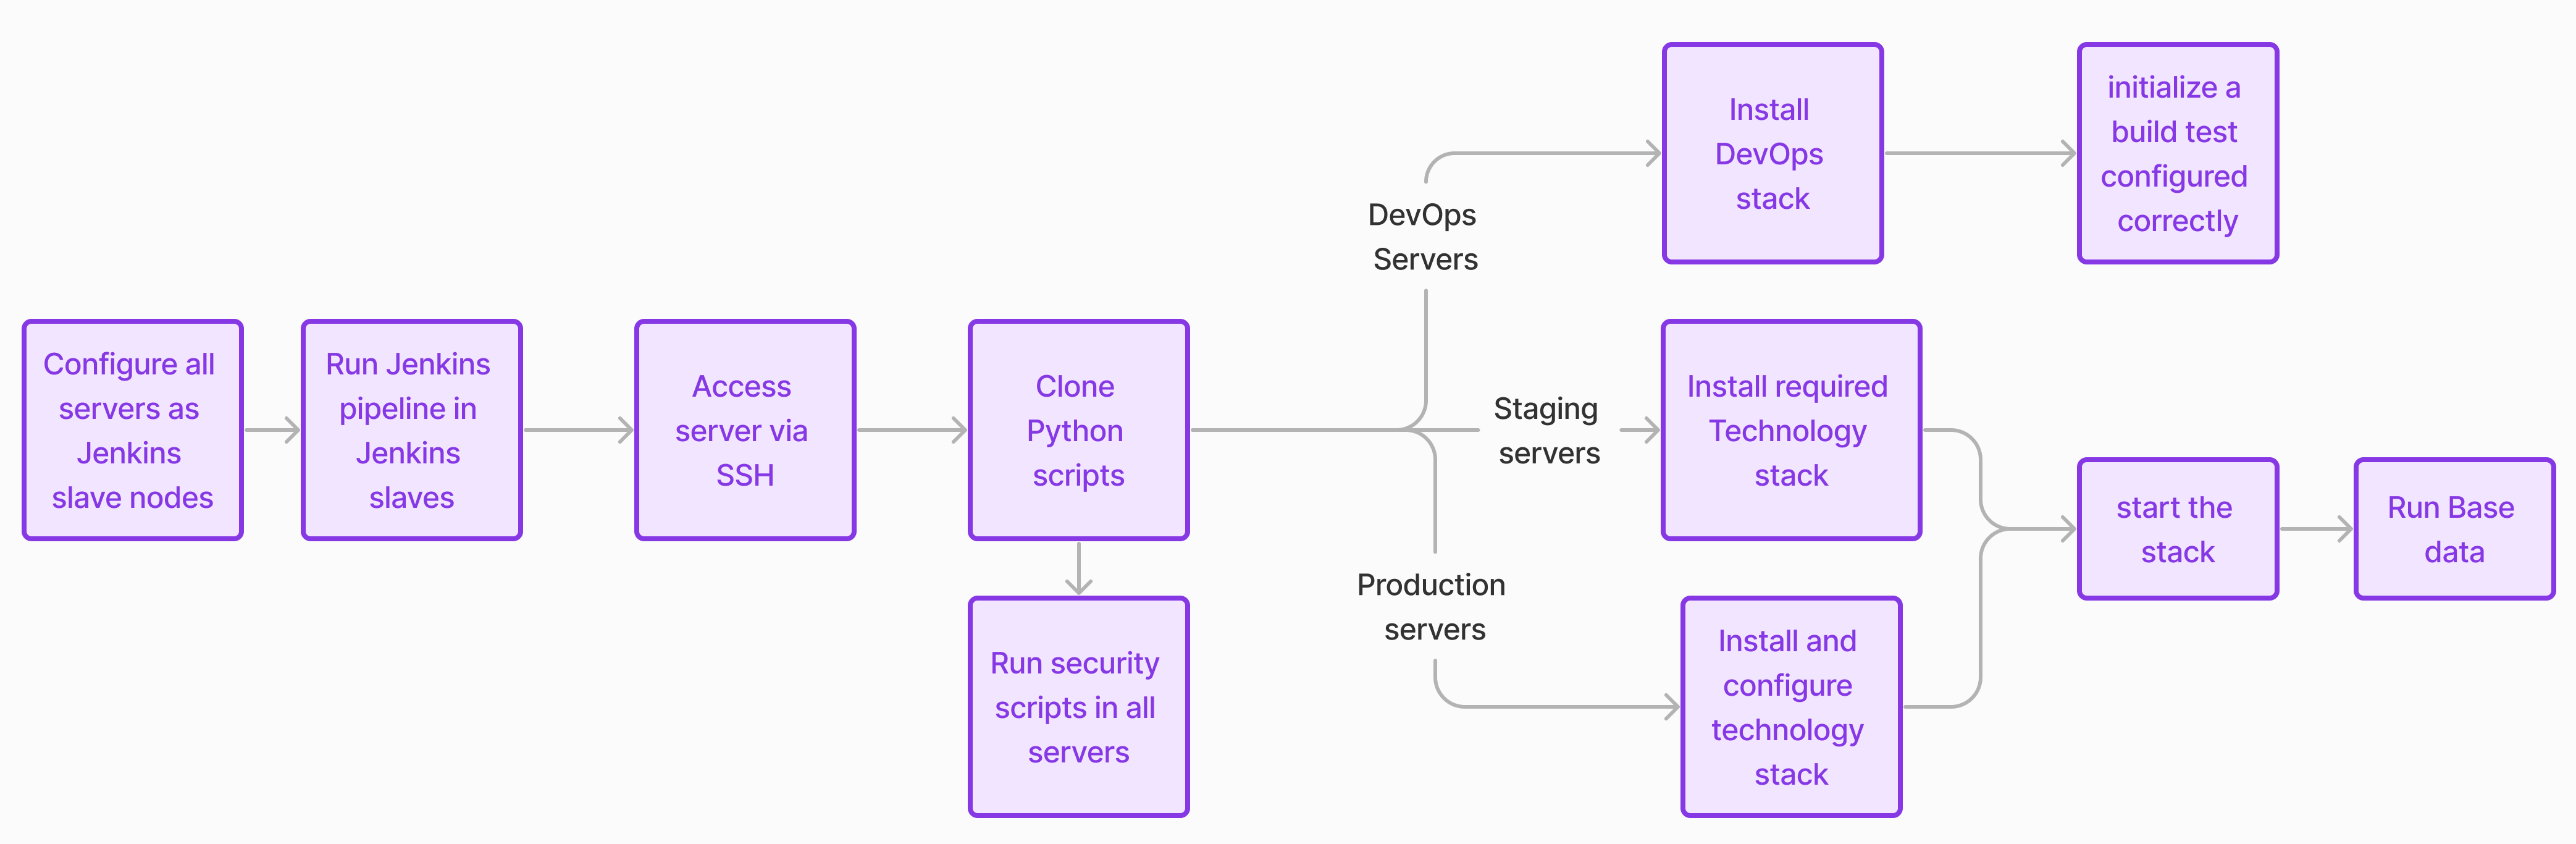
\includegraphics[width= 180mm, height = 80mm]{images/flowchart.png}
    \caption{Flowchart of Automation Processes}
    \label{fig:figure2_2}
\end{figure}
\section{Jenkins}
\par  Jenkins is an open source automation server. It helps automate the parts of software development related to building, testing, and deploying, facilitating continuous integration, and continuous delivery. It is a server-based system that runs in servlet containers such as Apache Tomcat. Jenkins plays a crucial role in automating various processes related to installation, configuration, security, monitoring, and management in DevOps workflows.

\subsection{Integration with Version Control}
\hspace{1cm} Jenkins seamlessly integrates with version control systems like Git, allowing for versioned scripts and configurations. This integration ensures that the latest versions of scripts are pulled from the repository during pipeline execution, promoting version control and traceability.

\subsection{Pipeline Orchestration}
\hspace{1cm} Jenkins pipelines orchestrate the entire process from start to finish. This includes steps such as checking out scripts, installing the necessary stack components, configuring the stack, executing Linux hardening scripts, and setting up data backups. Pipelines ensure that these tasks are executed in a specified sequence, reducing errors and ensuring consistency.

\subsection{Automated Script Execution}
\hspace{1cm} Jenkins facilitates the automated execution of Python automation scripts for installing and configuring the technology stack. By integrating these scripts into Jenkins pipelines, tasks that would otherwise require manual intervention, such as checking out scripts on servers and running them, are automated.


\subsection{One-Click Deployment}
\hspace{1cm} Jenkins enables one-click deployment through its web interface or API. This simplifies the deployment process, allowing users to trigger the entire automation workflow with a single click, as mentioned in the methodology.

\subsection{Monitoring and Visualization}
\hspace{1cm} Jenkins integrates with monitoring and visualization tools like Grafana, allowing for real-time monitoring of system metrics, backup status, and overall system health. This integration enhances visibility into critical metrics and provides insights for effective monitoring and management.

Overall, Jenkins streamlines and automates the DevOps processes involved in installing, configuring, securing, and monitoring technology stacks, making the entire workflow more efficient, reliable, and scalable.



\section{DevOps application stack}
\par

The DevOps application stack refers to the integrated set of software tools, technologies, and services used to automate and streamline the development, deployment, monitoring, and management processes within a DevOps environment. The appplications mentioned below need to be installed in DevOps servers.

\begin{figure}[ht]
    \centering
    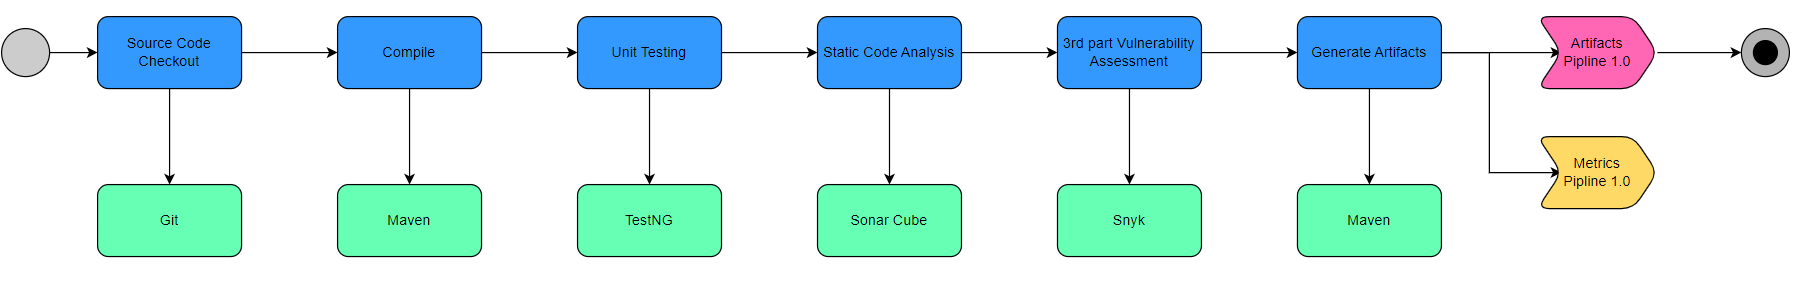
\includegraphics[width=180mm , height = 50mm]{images/devops stack.png}
    \caption{DevOps pipeline}
    \label{fig:figure2_2}
\end{figure}

\begin{itemize}
  


\item \textbf{Git} is a distributed version control system used for tracking changes in source code during software development. It allows multiple developers to collaborate efficiently by managing different versions of files and facilitating merging changes.

\item \textbf{Maven} is a build automation tool primarily used for Java projects to manage project dependencies, build processes, and project lifecycle management. It simplifies the build process by providing a standardized structure, known as Project Object Model (POM), which defines project configuration, dependencies, and build targets. Maven retrieves dependencies from central repositories, allowing developers to easily manage and share libraries across projects. It also supports various plugins for additional functionalities such as testing, packaging, and deployment, making it a popular choice for Java developers for efficient project management and automation.

\item \textbf{TestNG} is a testing framework designed for Java that facilitates the creation and execution of automated tests. It supports a wide range of testing scenarios, including unit, functional, integration, and end-to-end testing. TestNG offers features such as annotations, parameterized testing, test dependency management, and parallel test execution, enhancing test flexibility, readability, and scalability. It is widely used in the Java community for its robust testing capabilities and integration with build tools like Maven and continuous integration platforms like Jenkins.

\item \textbf{SonarQube} is an open-source static code analysis tool used for continuous inspection of code quality and security vulnerabilities. It analyzes code across multiple programming languages, identifying issues such as bugs, code smells, security vulnerabilities, and duplication. SonarQube provides detailed reports, metrics, and visualizations to help developers and teams improve code quality, maintainability, and reliability. It integrates seamlessly into the CI/CD pipeline, allowing for automated code analysis and enforcing code quality standards throughout the development lifecycle.

\item \textbf{PostgreSQL} is used with SonarQube for its scalability, reliability, performance, and security features, ensuring efficient storage and management of code analysis data. SonarQube officially supports PostgreSQL, making it an ideal choice as the database backend for organizations using SonarQube for code quality and security analysis.

 
\item \textbf{Snyk} is a developer-first security platform that helps organizations find, fix, and prevent vulnerabilities in open-source libraries and container images. It scans projects and dependencies for known security vulnerabilities and provides actionable insights to remediate issues. Snyk integrates with CI/CD pipelines to automate vulnerability scanning and remediation, ensuring that vulnerabilities are addressed early in the development process. Its continuous monitoring capabilities help organizations stay updated on new vulnerabilities and maintain a secure codebase.
\end{itemize}

\section{Deployment stack}
\par In this deployment architecture, incoming traffic first passes through a firewall that acts as a security barrier, filtering and allowing only authorized requests to proceed. Behind the firewall, HAProxy, a high-performance load balancer, distributes the incoming traffic across a cluster of Tomcat servers. These Tomcat servers host the application logic and handle client requests efficiently. The communication between HAProxy and the Tomcat server cluster is optimized for load balancing and fault tolerance, ensuring that the workload is evenly distributed and that the system remains highly available. Additionally, the Tomcat servers are interconnected with Percona XtraDB Cluster, ScyllaDB Cluster, and Redpanda Cluster, forming a robust backend infrastructure for data storage, processing, and messaging. This setup ensures scalability, reliability, and performance for handling diverse workloads and maintaining smooth operations of the overall system.


\begin{figure}[ht]
    \centering
    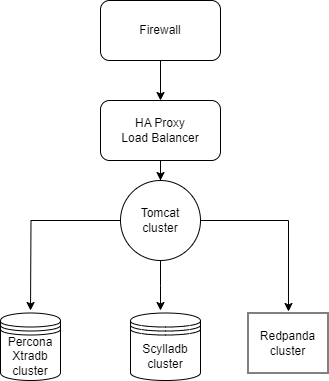
\includegraphics[width=120mm , height = 130mm]{images/deploy.drawio.png}
    \caption{Server Architecture}
    \label{fig:figure2_2}
\end{figure}

\par The main objective is to automate the deployment of this application architecture, including the installation and configuration of databases across multiple servers to form clusters. This automation streamlines the setup process, allowing for easy scaling by adding additional database servers to handle increasing loads efficiently. The focus is on creating a seamless infrastructure where Tomcat servers can dynamically distribute the workload among different database clusters, optimizing performance and ensuring high availability.

\begin{itemize}
\item \textbf{HAProxy} is a high-performance open-source load balancer that efficiently distributes incoming network traffic across multiple backend servers based on customizable rules and algorithms. It helps improve application performance, scalability, and reliability by evenly distributing workloads and managing server resources effectively.

\item \textbf{Apache Tomcat} is an open-source Java-based servlet container that provides a runtime environment for Java web applications. It serves as a web server capable of executing Java servlets and JavaServer Pages (JSP), handling HTTP requests, and generating dynamic content. Tomcat's architecture includes a core servlet container responsible for managing the lifecycle of servlets, along with additional components like Catalina for managing web applications, Coyote for handling HTTP requests, and Jasper for JSP processing, making it a versatile platform for hosting Java web applications.

\item \textbf{Percona XtraDB Cluster} is an open-source, high-availability MySQL clustering solution based on the Percona Server for MySQL. It is designed to provide high performance, scalability, and fault tolerance for database environments. Percona XtraDB Cluster uses synchronous replication between nodes, ensuring data consistency across the cluster while offering automatic node recovery and failover capabilities. Additionally, it supports features like multi-master replication, read and write scalability, and easy integration with existing MySQL applications, making it a robust choice for deploying highly available MySQL databases.

\item \textbf{ScyllaDB} is a distributed NoSQL database built for high performance and low-latency applications. It is designed as a drop-in replacement for Apache Cassandra, providing compatibility with Cassandra Query Language (CQL) and data models while offering superior performance. In a ScyllaDB cluster, data is distributed across multiple nodes for scalability and fault tolerance, with each node capable of handling reads and writes independently. The cluster employs a shared-nothing architecture, where each node operates autonomously and communicates through a gossip protocol for coordination and data replication. ScyllaDB's efficient design and integration with modern hardware technologies make it well-suited for real-time big data workloads and high-throughput applications.
\item \textbf{Redpanda} is a distributed streaming platform designed for high-performance, low-latency, and scalable data processing. It is built as an alternative to Apache Kafka, offering compatibility with Kafka APIs and tools while providing improved performance and reliability. In a Redpanda cluster, data streams are distributed across nodes for fault tolerance and horizontal scalability, making it suitable for real-time data streaming and event-driven applications.
\end{itemize}


\section{Monitoring Stack}
\par The automation process encompasses the installation and configuration of various service exporters such as MySQL, Scylla, Redpanda, PostgreSQL, Node, HAProxy, Jenkins, and others. These exporters facilitate the extraction of specific metrics and data from the respective services, making them accessible to Prometheus for centralized monitoring. Prometheus is then configured to collect metrics from these exporters, apply custom requirement alert rules, and store the data in a dedicated time series database configured to maintain data for at least 365 days. Furthermore, Grafana is automated for installation, and customized dashboards are set up to visualize the collected metrics from Prometheus, enabling effective monitoring and analysis of system performance and health. This end-to-end automation enhances operational efficiency, provides real-time insights, and supports proactive management of the entire infrastructure and services.

\begin{figure}[ht]
    \centering
    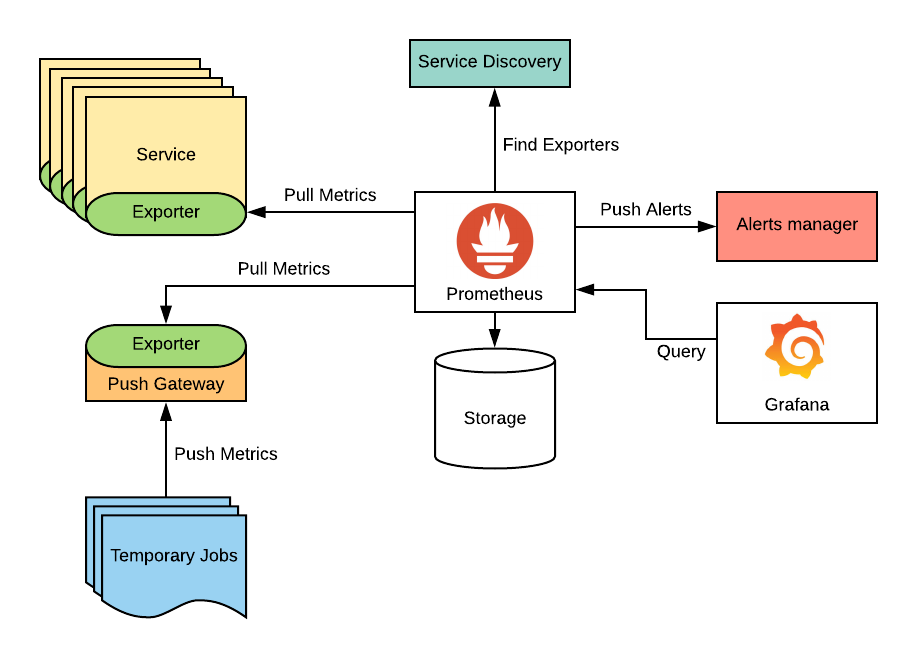
\includegraphics[width=140mm , height = 120mm]{images/monstack.png}
    \caption{Monitoring Stack Architecture}
    \label{fig:figure2_2}
\end{figure}

\begin{itemize}
\item \textbf{Service Exporters: }Service exporters in Prometheus are specialized exporters used for monitoring specific services or applications that don't expose Prometheus-compatible metrics natively. These exporters bridge the gap by translating service-specific metrics into a format that Prometheus can scrape and process. Examples include Node Exporter for system-level metrics, Blackbox Exporter for probing endpoints, and exporters for databases (e.g., MySQL, PostgreSQL) and cloud platforms (e.g., AWS, Azure) to monitor their performance and health metrics within Prometheus.
\item \textbf{Prometheus: }Prometheus is an open-source monitoring and alerting toolkit designed for collecting and processing metrics from various sources. It offers a multi-dimensional data model, powerful querying language (PromQL), and efficient storage for time-series data. Prometheus scrapes metrics from instrumented applications, services, and systems, providing insights into their performance and health.
\item \textbf{Prometheus Alertmanager: }Prometheus Alertmanager is a component that manages and handles alerts generated by Prometheus. It provides features like deduplication, grouping, and routing of alerts to different receivers (e.g., email, PagerDuty, Slack) based on predefined rules and configurations. Alertmanager enhances the monitoring experience by ensuring timely and effective response to critical events and incidents.
\item \textbf{Grafana: }Grafana is an open-source analytics and visualization platform that integrates with Prometheus and other data sources to create interactive and customizable dashboards. It enables users to create visual representations of metrics collected by Prometheus, helping teams to monitor and analyze system performance, identify trends, and gain actionable insights through graphs, charts, and alerts.
\end{itemize}


\section{Linux hardening}
\par Linux hardening involves implementing various security measures to protect a server from potential threats and vulnerabilities. This includes securing network services, managing user permissions, enabling firewall rules, applying system updates regularly, and configuring audit logs. By hardening Linux systems, organizations can reduce the attack surface, mitigate risks, prevent unauthorized access, and enhance overall system security. In the automated process, the Linux system hardening measures are validated using tools like Lynis. Lynis assesses the security posture of Linux systems by evaluating configuration settings, checking for security best practices adherence, and assigning a security score based on the findings. The requirement is that the Lynis score should be more than 85 percent to proceed with setting up the technology stack.

Additionally, the Lynis score is integrated as a metric in Prometheus, which collects and stores system metrics, including the Lynis score. This metric is then visualized in Grafana, providing a comprehensive view of the server's security status. This automated process not only ensures that the server meets security standards but also provides visibility into the security posture through Grafana dashboards, enabling proactive monitoring and management of system security.

 \section{Automating the Data Backup and Restoration}
\par To automate the data backup process in MySQL and ScyllaDB databases, we will schedule nightly backups at 2:00 am using cron jobs or scheduled tasks. These backup scripts will be designed to capture all necessary data and configurations from both MySQL and ScyllaDB databases, ensuring comprehensive backup coverage. Following the backup process, verification checks will be implemented to ensure data integrity. This includes automatically verifying the number of rows in MySQL tables and the number of columns in ScyllaDB tables within the backup files. Automated scripts or queries will handle these verification checks, comparing the counts in the backup files against the corresponding tables in the production databases.

Next, an automated restoration process will be set up on a separate server to restore the production backups of MySQL and ScyllaDB databases. This segregated server environment ensures a non-disruptive restoration process. Once the restoration is complete, another automated comparison will be conducted to verify the row/column counts between the restored databases and the production databases. If the counts match, indicating successful restoration, the metric will be exposed.

However, if discrepancies are detected during the comparison, indicating a potential issue with the restoration process, an alert will be triggered. The alerting mechanism will be integrated with Prometheus for monitoring purposes. In case of a mismatch in row/column counts, an alert will be sent out to all DevOps engineers via email or Slack channels, ensuring prompt notification and resolution of any backup or restoration issues. This comprehensive automation workflow streamlines the data backup, restoration, verification, and monitoring processes, enhancing data reliability and operational efficiency.

\newpage
\chapter{Implementation}
\section{Data Preprocessing}
\par The initial phase of the Intelligent Search Assistant project involves processing a multitude of documents in various formats, including PDFs, Word documents, and plain text files. This diverse range of sources ensures comprehensive data intake for the system. Leveraging the robust capabilities of the LangChain framework, the system meticulously parses the text from these documents, breaking them down into manageable segments. This segmentation not only enhances processing efficiency but also facilitates a more granular understanding of the content, laying the foundation for subsequent steps in the information retrieval process.

\section{Embedding Generation}
\par Once the text segments are parsed, the system proceeds to transform them into embeddings, which serve as numerical representations of the semantic meaning of the text. This transformation is facilitated by the sophisticated Sentence Transformer technique, which excels in capturing contextual information and semantic relationships within the text segments. By generating embeddings rich in information and context, the system lays the groundwork for efficient storage and retrieval of relevant information, setting the stage for seamless user interactions.

\section{Vector Storage}
\par Efficient storage of embeddings is paramount for ensuring quick access to relevant information during user interactions. To this end, the Intelligent Search Assistant leverages LangChain's Chroma vector storage mechanism. This mechanism not only optimizes memory usage but also enhances retrieval speed, thanks to its structured organization of embeddings. By efficiently storing embeddings in a manner conducive to rapid retrieval, the system ensures responsiveness and effectiveness in addressing user queries and prompts, thereby enhancing the overall user experience.

\section{User Query Preocessing}
\par As users submit queries or prompts, the system springs into action, leveraging the Conversation Retrieval Chain to retrieve relevant documents or context. This chain seamlessly integrates retrieval techniques tailored to user input, drawing upon the stored embeddings in the Chroma vector database. By ensuring that the retrieved documents or context are contextually relevant to the user's query, the system enhances the accuracy and usefulness of the responses provided, laying the groundwork for personalized and effective interaction.
\begin{figure}[ht]
    \centering
    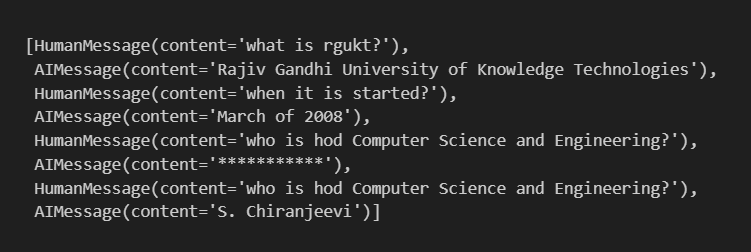
\includegraphics[width=125mm , height = 90mm]{images/rgukt-01.png}
    \caption{Q and A On Rgukt Website}
    \label{fig:figure2_2}
\end{figure}

% \begin{figure}[ht]
%     \centering
%     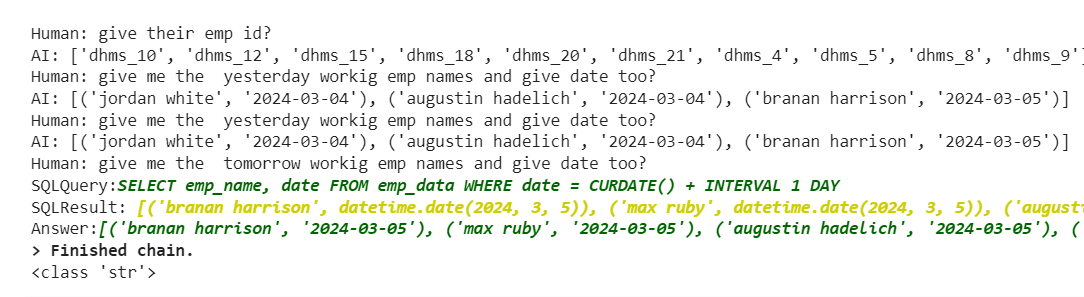
\includegraphics[width=215mm , height = 70mm]{db1.png}
%     \caption{Natural Question on the SQL Database}
%     \label{fig:figure2_2}
% \end{figure}






\newpage
\section{Google Drive Integration}
\par Google Drive integration in the Intelligent Search Assistant facilitates effortless access to files stored in users' Google Drive accounts, enhancing the efficiency of information retrieval processes. The integration begins with OAuth2 authentication to establish a secure connection with Google Drive, ensuring users' data privacy and security. Upon authentication, the system interacts with the Google Drive API to retrieve a list of files and folders, enabling users to specify the target folder for downloading files. Utilizing retrieved file metadata, the system initiates the download process from the specified folder, handling various file formats seamlessly, including documents, spreadsheets, images, and presentations.

Furthermore, the system intelligently determines the appropriate file format and extension based on the MIME type provided by Google Drive, supporting a wide range of formats such as CSV, Excel, and DOCX. To enhance reliability, a retry mechanism is incorporated for file downloads, automatically retrying the download process in case of network issues or timeouts. Additionally, robust error handling mechanisms are implemented to gracefully manage exceptions and communicate errors to users, ensuring a smooth user experience. By seamlessly integrating with Google Drive, the Intelligent Search Assistant empowers users to leverage their existing file repositories for enhanced information retrieval and analysis, thereby facilitating a streamlined workflow and improving productivity.
\hspace{10pt}

\begin{figure}[ht]
    \centering
    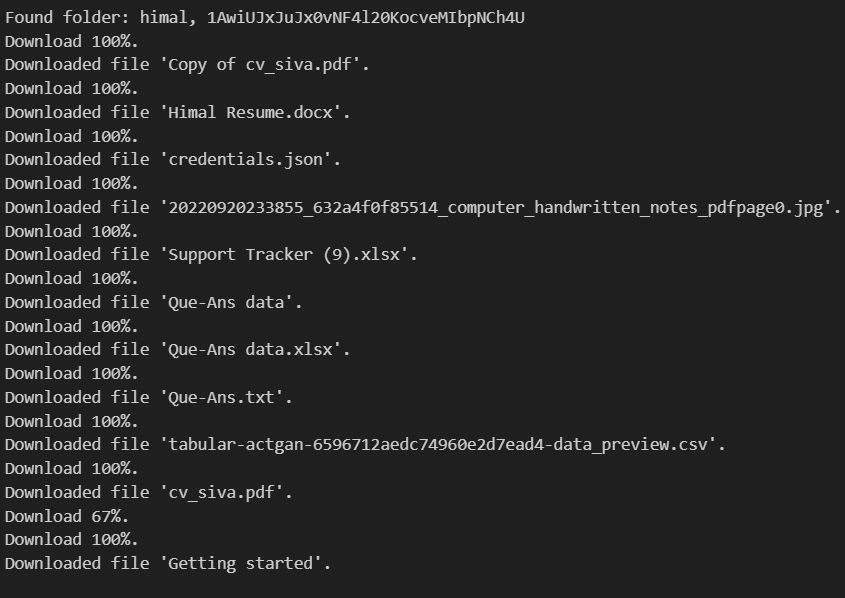
\includegraphics[width=145mm , height = 110mm]{images/google-drive.png}
    \caption{Integrating Google-drive data With Intelligent Search Assistant}
    \label{fig:figure2_2}
\end{figure}

\newpage
\chapter{Result}
\section{Result}
\par The Intelligent Search Assistant successfully integrates retrieval-augmented generation (RAG) techniques with large language models (LLMs) to deliver personalized and contextually relevant responses to user queries. Through the streamlined process of data preprocessing, embedding generation, and vector storage, the system efficiently organizes and retrieves information from diverse sources, including documents, websites, and multimedia content. Leveraging the LangChain framework and the Sentence Transformer technique, the system transforms textual data into compact embeddings, facilitating quick retrieval and response generation.

Moreover, the integration with Google Drive enables seamless access to users' files, enhancing the breadth and depth of information available for retrieval. By intelligently parsing file metadata and employing robust download mechanisms, the system ensures smooth and reliable access to various file formats, including documents, spreadsheets, images, and presentations. The result is an intelligent search assistant that empowers users to access and analyze information from their Google Drive repositories with ease, ultimately improving productivity and facilitating informed decision-making.

\section{Sample Output Screenshots}

\begin{figure}[ht]
    \centering
    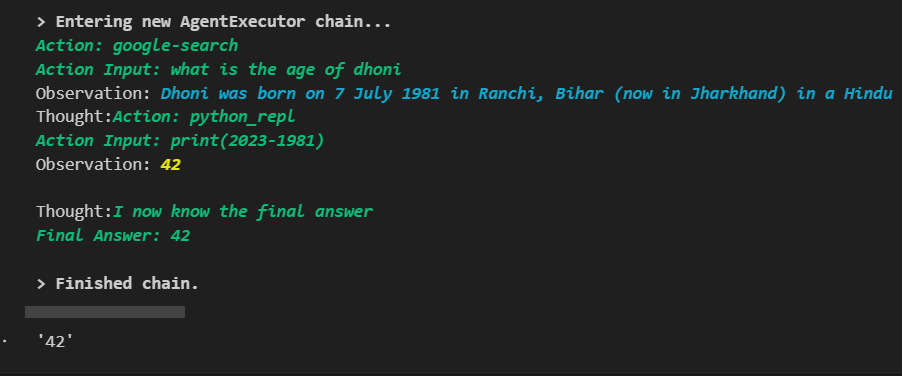
\includegraphics[width=145mm , height = 110mm]{Dhoni.png}
    \caption{Making LLM models Up to date with Lagnchain agent}
    \label{fig:figure2_2}
\end{figure}


\section{Requirements}
\subsection{Software Requirements}
\begin{itemize}
\item{LangChain}
\item{Embeddings Techniques}
\item{Retrieval-Augmented Generation (RAG) techniques}
\item{Large Language Models (LLMs)}
\item{Vector Databases}
\item{Python}
\end{itemize}

\subsection{Hardware Requirements}

\begin{itemize}
\item{Modern Operating System}
\item{4 GB RAM}
\item{10 GB Free Disk Space}
\item{X86 64-bit CPU(Intel/AMD Architecture)}
\end{itemize}




\newpage
\chapter{Future Scope}
\textbf{    Integrating More Data Storage Platforms:} By incorporating additional data storage platforms like Slack, OneDrive, and Dropbox, you can enhance the accessibility and versatility of your Intelligent Search Assistant, allowing users to retrieve information from a wider range of sources.

\textbf{Implementing Efficient Chunking Techniques:} Introducing advanced chunking techniques such as semantic chunking can improve the organization and retrieval of information within the system, leading to more accurate and relevant search results for users.


\textbf{Creation of Web Application Using ChainLit Python Framework:} Developing a web application using the ChainLit Python framework can make your Intelligent Search Assistant more accessible to users across different platforms and devices, expanding its reach and usability.

\textbf{Local Project with LLM Model Download:} Enable users to run the Intelligent Search Assistant locally by downloading the LLM model, providing greater control and flexibility, especially in environments with limited internet access or privacy concerns.

\textbf{Converting Application into No-Code Platform:} TTransform the application into a no-code platform, allowing users to easily build customized assistants using drag-and-drop functionality, democratizing access to AI-powered information retrieval tools for users with varying technical expertise.
\newpage
\chapter{Conclusion}
\hspace{20pt}In conclusion, the Intelligent Search Assistant represents a significant advancement in information retrieval systems, leveraging cutting-edge technologies such as LangChain, large language models (LLMs), and retrieval-augmented generation (RAG) techniques. Through seamless integration with various data sources including Google Drive and robust document preprocessing methods, the system offers users a personalized and efficient means of accessing relevant information. The future scope of the project, including integration with additional storage platforms, implementation of advanced chunking techniques, and conversion into a no-code platform, promises further enhancements in usability and accessibility. Overall, the project showcases the potential of AI-driven solutions to revolutionize user interaction and streamline information retrieval processes.

\newpage
\chapter{Refernece}
\begin{itemize}
\item{https://python.langchain.com/docs/}
\item{https://cloud.google.com/docs}
\item{https://www.analyticsvidhya.com/blog/2023/09/retrieval-augmented-generation-rag-in-ai/}
\item{https://docs.trychroma.com/usage-guide)}
\item{https://huggingface.co/docs}
\item{https://docs.llamaindex.ai/en/stable/}
\end{itemize}


\end{document}